\documentclass[paper=a4, fontsize=11pt]{scrartcl}
\usepackage[T1]{fontenc}
\usepackage{fourier}

\usepackage[english]{babel}                             % English language/hyphenation
\usepackage[protrusion=true,expansion=true]{microtype}  
\usepackage{amsmath,amsfonts,amsthm} % Math packages
\usepackage[pdftex]{graphicx} 
\usepackage{url}
\usepackage[section]{placeins}


%%% Custom sectioning
\usepackage{sectsty}
\allsectionsfont{\centering \normalfont\scshape}
\usepackage{color}
\usepackage{color,soul}

%%% Custom headers/footers (fancyhdr package)
\usepackage{fancyhdr}
\pagestyle{fancyplain}
\fancyhead{}                      % No page header
\fancyfoot[L]{}                     % Empty 
\fancyfoot[C]{}                     % Empty
\fancyfoot[R]{\thepage}                 % Pagenumbering
\renewcommand{\headrulewidth}{0pt}      % Remove header underlines
\renewcommand{\footrulewidth}{0pt}        % Remove footer underlines
\setlength{\headheight}{13.6pt}


%%% Equation and float numbering
\numberwithin{equation}{section}    % Equationnumbering: section.eq#
\numberwithin{figure}{section}      % Figurenumbering: section.fig#
\numberwithin{table}{section}       % Tablenumbering: section.tab#


%%% Maketitle metadata
\newcommand{\horrule}[1]{\rule{\linewidth}{#1}}   % Horizontal rule

\title{
    %\vspace{-1in}  
    \usefont{OT1}{bch}{b}{n}
    \normalfont \normalsize \textsc{Carnegie Mellon University - Computational Biology Department} \\ [25pt]
    \horrule{0.5pt} \\[0.4cm]
    \huge Active Learning for Drug Selection\\ on Identified Target Protein \\
    \horrule{2pt} \\[0.5cm]
}
\author{
  Christine Baek\\
  \normalsize\texttt{christib@andrew.cmu.edu}
  \and
  Qi Chu\\
  \normalsize\texttt{qchu@andrew.cmu.edu}
  \date{}
}
\date{}


\newcommand{\TODO}[1]{\textcolor{red}{\textbf{TODO: } #1}}

%%% Equation and float numbering
\numberwithin{equation}{section}    % Equationnumbering: section.eq#
\numberwithin{figure}{section}      % Figurenumbering: section.fig#
\numberwithin{table}{section}       % Tablenumbering: section.tab#
\usepackage[T1]{fontenc}
\usepackage[utf8]{inputenc}
\usepackage{tabularx,ragged2e,booktabs,caption}
\newcolumntype{C}[1]{>{\Centering}m{#1}}
\renewcommand\tabularxcolumn[1]{C{#1}}







%%% Begin document
\begin{document}
\maketitle
\section{Introduction}
In this project, we explore three datasets of different noise and/or labels, for identification of compounds that bind to specific target protein. We first perform feature selection using $\chi^2$ test, then adopt the \textit{largest positive score}~\cite{ref:warmuth} for active learning strategy, and SVM for model learning. We also perform a gradient experiment to learn the optimal balance for allocating queries between feature selection and model learning.



\section{Methods}

Input :
\begin{itemize}
\item Training data consists of 4000 training instances, each with 1000 features and true label 
\item Test data consists of 1000 testing instances, each with 1000 features and true label
\item Blind prediction data consists of 1000 instances, each with 1000 features
\item Each data(row) represents potential compound that may bind to the target
\item Each feature(column) represents structural or chemical 
\end{itemize}




As with real world drug target screening, we began with assumption that only an extremely small fraction of compounds will bind to the target. Also, only a small fraction of the features would be relevant in predicting the label (are actual sites that the drug can potentially bind to). Our challenge is to first find which features are relevant in accurately predicting whether the compound will bind to the target or not, and then learning on those features.


We performed gradient experiment, and measured the performance based on the number of queries made between initial learning and active learning, as the total number of queries is capped at 2500. Our predictions are then compared against random learner, as well as 0-guess, which predicts inactivity (label=0) for all compounds. 


\subsection{Learning Strategy}

Because of the imbalanced dataset (only small portion of the molecules actually bind to target), it would have been dangerous to use active learning strategy without any prior. We decided to split our learning into two different phases : Initial and Active. During initial learning, we randomly select molecules without any assumptions or selection criteria, other than choosing molecules we have not seen before. We perform feature selection during this phase. Once initial learning is over, we begin the active learning phase where points are selected per \textit{largest positive} strategy as discussed in ~\cite{ref:warmuth}, elaborated below. Total number of queries made during both initial and active phase total 2500, the allotted budget. 


\subsubsection{Initial Feature Selection}

Randomly chosen molecules are queried for their label and features. This initial phase is important in learning which features are relevant, in order to build a more relevant model. While data has been omitted, our previous attempts without explicit feature selection has returned low F1 score as well as error rate. 

\subsubsection{Active Compound Selection}

We used selection strategy of \textit{largest positive score} which performed the best in ~\cite{ref:warmuth}. Given that most compounds are inactive and would be predicted to be 0, this strategy searches for the compounds that are active and effective in discovering potentially active compounds. Given our goal of drug discovery for our target, false positives (drugs that are classified as binding to target, but does not) can be tolerated within reason, but false negatives are potentially costly. We do not expend our limited number of queries for looking up inactive compounds, but instead dedicate our efforts towards finding potentially active compounds which are far and few between. \textit{Largest positive} score compound is selected by computing a \textit{score} of activity based on signed distance from the SVM hyperplane. Note that this strategy works for our purpose of finding as many positive molecules that bind to drug target, but a different strategy such as choosing compounds near boundary may be more suited for studying the structure-activity relationship ~\cite{ref:warmuth}

\subsection{Classifier Strategy}

\TODO{elaborate}


SVM was chosen as our classifier for multiple reasons. SVM finds a hyperplane that maximizes the distance between the nearest data (support vectors) and the hyperplane. Given the high dimension of our input data (1000 features) with assumption of linear separability, it was important that a classifier that scales easily to high dimension, with no local optima. SVM separates inactive from active compounds by using maximum margin hyperplane for decision boundary. 
Gaussian kernel (default) was used for training. 


\section{Results}

Gradient experiment was performed for varying number of queries divided between the initial learning (feature selection) and active learning (model learning). Graphs for each section (difficulty) include the best performing division of queries, but full data is available 

\subsection{Easy}


\begin{figure}[!htb]
  \centering
  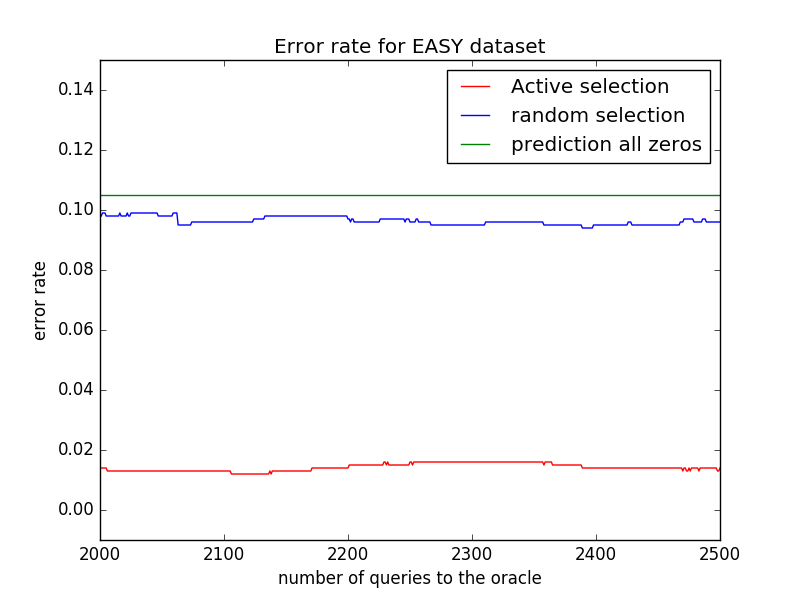
\includegraphics[scale = 0.5]{figures/error_easy.png}
      \caption{Error rate of easy test set plotted against number of queries made to oracle}
      \label{easyerror}
\end{figure}


\begin{figure}[!htb]
  \centering
  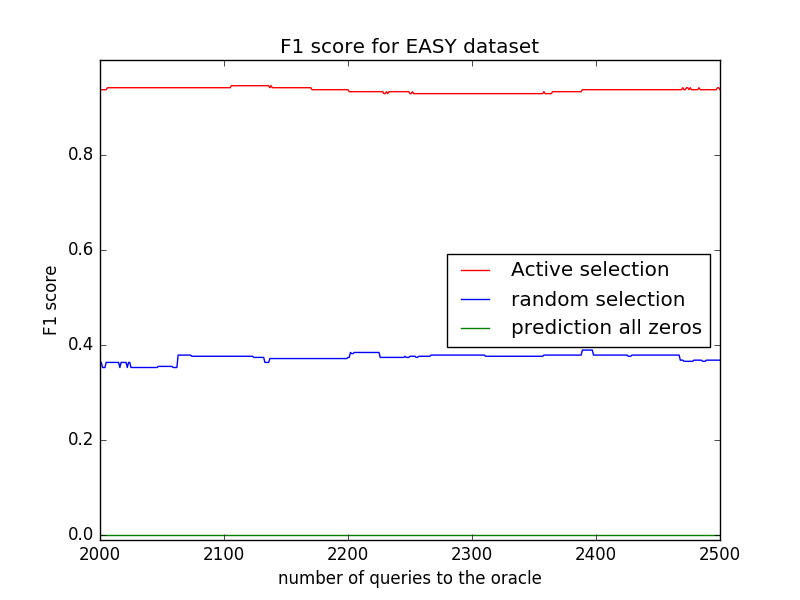
\includegraphics[scale = 0.5]{figures/f1_easy.png}
      \caption{F1 Score of easy test set plotted against number of queries made to oracle}
      \label{easyf}
\end{figure}



\FloatBarrier
\subsection{Moderate}

\begin{figure}[!htb]
  \centering
  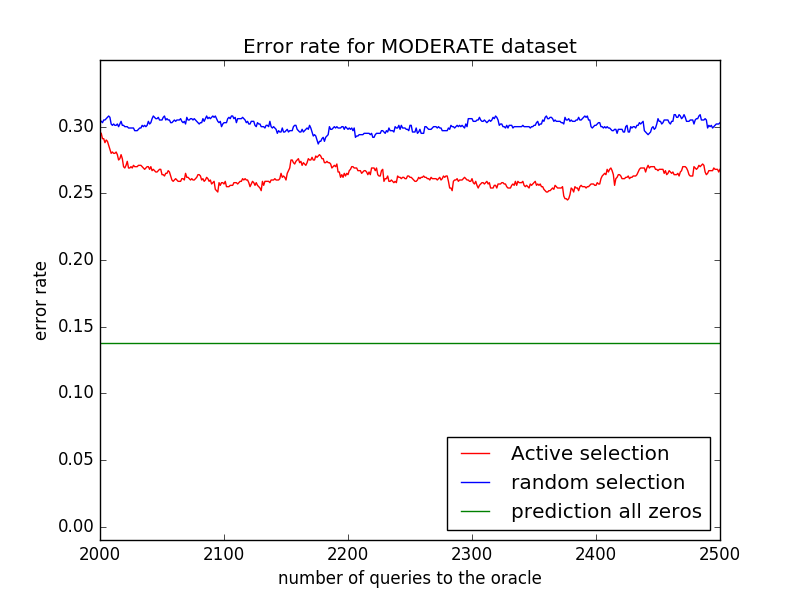
\includegraphics[scale = 0.5]{figures/error_moderate.png}
      \caption{Error rate of moderate test set plotted against number of queries made to oracle}
      \label{moderror}
\end{figure}

\begin{figure}[!htb]
  \centering
  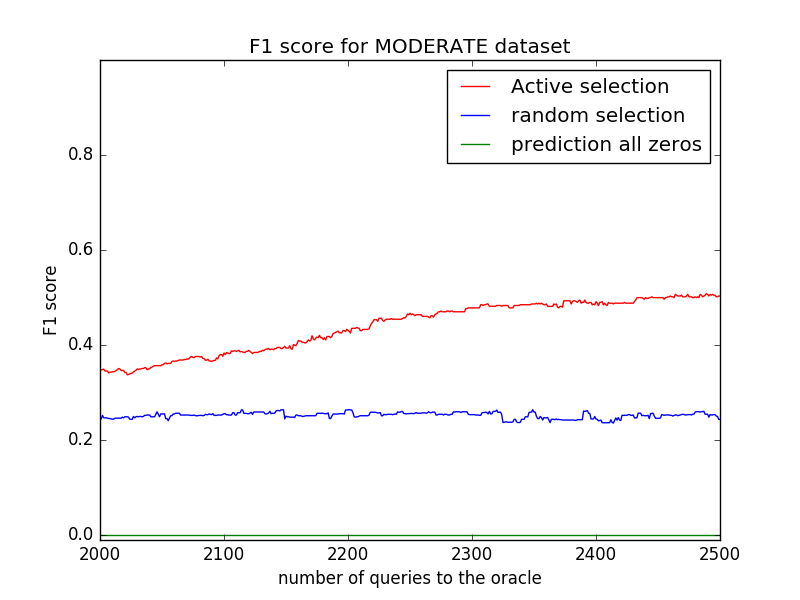
\includegraphics[scale = 0.5]{figures/f1_moderate.png}
      \caption{F1 score of moderate test set plotted against number of queries made to oracle}
      \label{modf}
\end{figure}
\FloatBarrier
\subsection{Difficult}


\begin{figure}[!htb]
  \centering
  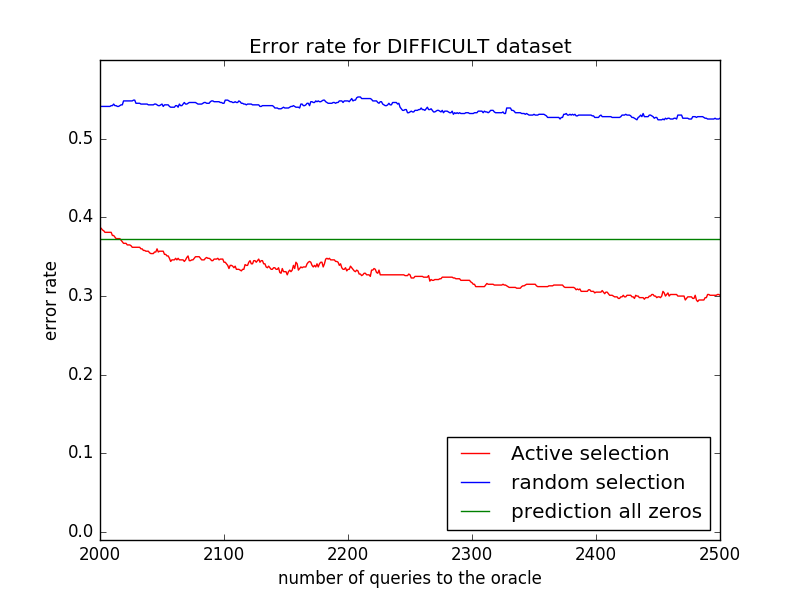
\includegraphics[scale = 0.5]{figures/error_difficult.png}
      \caption{Error rate of difficult test set plotted against number of queries made to oracle}
      \label{harderror}
\end{figure}

\begin{figure}[!htb]
  \centering
  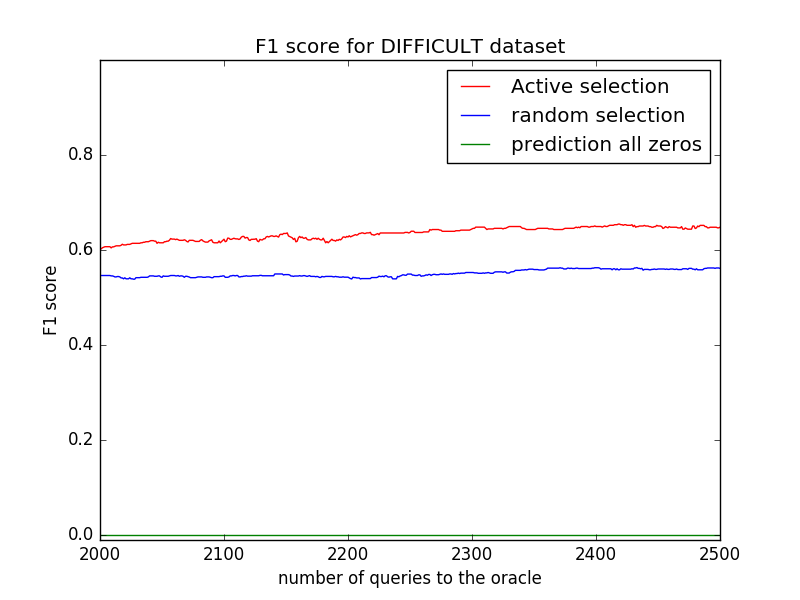
\includegraphics[scale = 0.5]{figures/f1_difficult.png}
      \caption{F1 score of difficult test set plotted against number of queries made to oracle}
      \label{hardf}
\end{figure}

\FloatBarrier

\begin{minipage}{\linewidth}
\smallskip
\centering
\captionof{table}{F1 score of various parameters} \label{f1table} 
\begin{tabular}{ p{2in} C{.85in} *4{C{.7in}}}\toprule[1.5pt]
\# of queries - Initial Learning & 500 & 1000 & 1500 & 2000  \\ \toprule[1.5pt]
\# of queries - Active Learning & 2000 & 1500 & 1000 & 500  \\ \bottomrule[1.25pt]
EASY                        & 0.6409                             & 0.6328                              & 0.9375                              & 0.9375                              \\
MODERATE                    & 0.2625                             & 0.4365                              & 0.4686                              & 0.5034                              \\
DIFFICULT(pos. v.s. neg.)   & 0.4286                             & 0.5133                              & 0.5346                              & 0.6481\\
\bottomrule[1.25pt]
\end{tabular} \par \bigskip
F1 score for 3 different input data, with gradient of initial vs active learning query division. 
This table shows the F1 score of each test data after the model had been trained on varying number of queries for Initial Learning (feature selection) and active learning (model learning). 
\end{minipage}
\FloatBarrier

\begin{minipage}{\linewidth}
\smallskip
\centering
\captionof{table}{Error rate of various parameters} \label{errortable} 
\begin{tabular}{ p{2in} C{.85in} *4{C{.7in}}}\toprule[1.5pt]
\# of queries - Initial Learning & 500 & 1000 & 1500 & 2000  \\ \toprule[1.5pt]
\# of queries - Active Learning & 2000 & 1500 & 1000 & 500  \\ \bottomrule[1.25pt]
EASY                          & 0.065                              & 0.065                               & 0.014                               & 0.014                               \\
MODERATE                      & 0.191                              & 0.142                               & 0.161                               & 0.146                               \\
DIFFICULT(pos. v.s. neg.)     & 0.622                              & 0.346                               & 0.375                               & 0.301                               \\
\bottomrule[1.25pt]
\end{tabular} \par \bigskip 
Error rate for 3 different input data, with gradient of initial vs active learning query division.
This table shows the error rate of each test data after the model had been trained on varying number of queries for Initial Learning (feature selection) and active learning (model learning). 
\end{minipage}
\FloatBarrier



\section{Conclusion}

\TODO{briefly summarize}


\begin{thebibliography}{1}

%\bibitem{ref:cal}
%Cohn, Atlas, Ladner, \emph{Improving  Generalization  with  Active  Learning},  Machine Learning May 1994, Volume 15, Issue 2, p 201-221

%\bibitem{ref:dhm}
%5S. Dasgupta, D. Hsu, C. Monteleoni, \emph{A general agnostic active learning algorithm}, NIPS, 2008 

%\bibitem{ref:twoface}
%S. Dasgupta, \emph{Two faces of active learning},  \texttt{http://cseweb.ucsd.edu/$\sim$dasgupta/papers/}, 2010

\bibitem{ref:warmuth}
Warmuth, Liao, Ratsch, Mathieson, Putta and Lemmen, \emph{Active Learning with Support Vector Machines in the Drug Discovery Process}, J. Chem. Inf. Comput. Sci. 2003, 43, 667-673

\end{thebibliography}


\end{document}